\chapter{Discrete two-body reactions}
\label{Sec:2-body}
This section describes how the contribution to the transfer matrix
is calculated for data consisting of probability densities for
the cosine of the angle of deflection in discrete 2-body reactions.
In this case, the probability densities are always given in 
the center-of-mass frame.
Because
the transfer matrices are defined in terms of laboratory
coordinates, the computations involve a boost.

For all except very light-weight targets, the mapping from
center-of-mass to laboratory coordinates is usually done using 
Newtonian mechanics.  The discussion given here is therefore
Newtonian.  A relativistic treatment is presented in Appendix~\ref{Appendix-relativity}.
The choice of Newtonian or relativistic mechanics is determined by
the value of the \textsf{kinetics} input parameter to \gettransfer\ as
explained in Section~\ref{Sec:relativistic}.  Of course, relativistic mechanics must
be used if either the incident particle or the outgoing particle is a
photon.

For discrete 2-body reactions,  the center-of-mass energy of the emitted particle
is determined by the energy $E$ of the incident particle.  Consequently, the
energy-angle probability density $\picm(\Ecm', \mucm \mid E)$ in the
center-of-mass frame is given by
\begin{equation}
  \picm(\Ecm', \mucm \mid E) =
  g( \mucm \mid  E) \, \delta( \Ecm' - \Psi( E ) )
  \label{prob_cm}
\end{equation}
for the function~$\Psi$ given below in Eq.~(\ref{E_cm}).  
From here on, the energy~$E$ and direction cosine~$\mu$
of the outgoing particle will be marked with the subscript ``lab'' or ``cm'' to
indicate that the variable is in the laboratory or center-of-mass frame.

Because of Eq.~(\ref{prob_cm}), the data for discrete 2-body reactions consist
of angular probability densities $g( \mucm \mid E)$ given in the 
center-of-mass frame, either as a 2-dimensional table 
for given incident energy~$E$ and direction cosine~$\mucm$
or as Legendre coefficients $c_\ell(E)$ for
\begin{equation}
  g( \mucm \mid  E) =
  \sum_\ell 
  \left(
     \ell + \frac{1}{2}
  \right)
    c_\ell(E)P_\ell( \mucm ).
  \label{cmLegendre}
\end{equation}

This section begins with an overview of Newtonian mechanics
for discrete 2-body problems.  In particular, the form of the function
$\Psi$ in Eq.~(\ref{prob_cm}) is derived, as is the boost from the
center-of-mass to the laboratory frame.  The section closes
with an examination of the use of angular probability data 
$g( \mucm \mid E)$ in the computation of the integrals
Eqs.~(\ref{Inum}) and~(\ref{Ien}) used in the calculation of the
transfer matrix.  

\section{Newtonian mechanics of discrete 2-body reactions}
\label{Sec:2-body-Newton}
Only a summary of the results is given here; for more information,
see the reference~\cite{endep}.  A relativistic treatment is
developed in Appendix~\ref{Appendix-relativity}.  It is assumed that the target is at rest 
and that the incident particle has
energy $E$ in laboratory coordinates.

The following
notations are used for the masses of the particles involved:\\
 \Input{$\myi$,}{  the mass of the incident particle,}\\
 \Input{$\mtarg$,}{ the mass of the target,}\\
 \Input{$\myo$,}{ the mass of the emitted particle,}\\
 \Input{$\mres$,}{ the mass of the residual.}\\
For the conversion
between center-of-mass and laboratory coordinates, define
the mass ratios
$$
  \gamma = \frac
    { \myi \myo }
    { ( \myi + \mtarg )^2 },
$$
$$
   \beta = \frac
    { \mres }
    { \myo + \mres },
$$
and
$$
   \alpha = \frac
    {\beta \mtarg}
    { \myi + \mtarg }.
$$

Velocity vectors are printed in bold face $\textbf{V}$ with
magnitude (speed) in math italics
$$
  V = | \textbf{V} |.
$$

For a target at rest and an incident particle with
energy $E$ in laboratory coordinates, the center of mass
moves in the direction of motion of
the incident particle with velocity $\Vtrans$ having magnitude squared 
\begin{equation}
  \vtrans^2 = \Vtrans^2 =
    \frac{ 2\myi  E}
    { ( \myi + \mtarg )^2 }.
  \label{Vtrans-length}
\end{equation}

The reaction may have a nonzero energy value $Q$, arising
for example from the excitation level of the target
and/or residual nucleus in inelastic scattering.  A nonzero
$Q$ value may also arise from the
mass difference in a knock-on reaction.  
It follows from conservation of energy and momentum that in
center-of-mass coordinates the energy of the emitted
particle is given by
\begin{equation}
  \Ecm' = \Psi( E ) = \alpha E + \beta Q.
  \label{E_cm}
\end{equation}
This defines the function $\Psi$ appearing in Eq.~(\ref{prob_cm}).
The speed of the outgoing particle in the
center-of-mass frame is
\begin{equation}
  \vcm' = |\Vcm'| = \sqrt{ \frac{ 2\Ecm' }{\myo} }.
    \label{V-cm-outgoing}
\end{equation}
It follows from Eq.~(\ref{E_cm}) that for an endothermic
reaction ($Q < 0)$, the threshold is at
$$
  E = \frac{-\beta Q}{\alpha}.
$$ 

\subsection{The boost to the laboratory frame}
As illustrated in Figure~\ref{Fig:2-body-boost}, the boost from center-of-mass
to laboratory coordinates is obtained by adding the velocities
\begin{equation}
  \Vlab' = \Vtrans + \Vcm'.
 \label{V-lab-2-body}
\end{equation}
Consequently, the energy of the outgoing particle in the
laboratory frame is
$$
  \Elab' = \frac{ \myo {\Vlab'}^2 }{2} =
        \frac{ \myo }{2}
        ( \vtrans^2 + {\vcm'}^2 + 2\Vtrans \cdot \Vcm' ).
$$
In terms of the notation Eq.~(\ref{E_cm}) and
\begin{equation}
  \Etrans' = \frac{ \myo \vtrans^2 }{2} =
  \gamma E,
  \label{E_trans}
\end{equation}
this equation takes the form
\begin{equation}
  \Elab' = \Etrans' + \Ecm' + 2 \mucm \sqrt{ \Etrans' \Ecm' }.
  \label{E_lab}
\end{equation}
Here, $\mucm$ is the direction cosine defined by the
relation
$$
   \Vtrans \cdot \Vcm' = \mucm \vtrans \vcm'.
$$
 
\begin{figure}
% mapping to laboratory coordinates
\begin{center}

\begin{tikzpicture}
% the triangle
  \draw[-{>[scale=2.5,
          length=5,
          width=3]},line width=0.4pt] (0, 0) -- (7.5, 3);
  \draw[-{>[scale=2.5,
          length=5,
          width=3]},line width=0.4pt] (0, 0) -- (6, 0);
  \draw[-{>[scale=2.5,
          length=5,
          width=3]},line width=0.4pt] (6, 0) -- (7.5, 3);
 % \draw[->, stealth, line width=0.4pt] (6, 0) -- (7.5, 3);
\draw (6, 0) -- (7.8, 0);
  \draw ( 1.2, 0) arc (0: 21.8: 1.2);
  \draw (6.8, 0) arc (0: 63.43: 0.8);
% labels
  \node [below] at (3.5, -0.15) {$\Vtrans$};
  \node [above] at (3.6, 1.7) {$\Vlab'$};
  \node [right] at (6.9, 1.6) {$\Vcm'$};
  \node [right] at (1.3, 0.4) {$\cos^{-1} \mulab$};
  \node [right] at (6.7, 0.6){$\cos^{-1} \mucm$};
\end{tikzpicture}
\caption{Newtonian mapping to laboratory coordinates}
\label{Fig:2-body-boost}
\end{center} 

\end{figure}

It is also necessary to determine the direction cosine $\mulab$ in
the laboratory frame for
$$
     \Vtrans \cdot \Vlab' = \mulab \vtrans \vlab'.
$$
This is most easily derived from the trigonometry in Figure~\ref{Fig:2-body-boost}
$$
  \mulab  \vlab' = 
   \vtrans + \mucm \vcm'.
$$
In terms of the energies defined in Eqs.~(\ref{E_cm}), (\ref{E_trans}),
and~(\ref{E_lab}), this relation takes the form
\begin{equation}
  \mulab  = \frac
   { \sqrt{ \Etrans' } + \mucm \sqrt{ \Ecm'} }
    {\sqrt{\Elab'}}
    \quad \text{if $\Elab' > 0$.}
  \label{get_mu}
\end{equation}

It is clear from Eq.~(\ref{V-lab-2-body}) that 
$$
  \Elab' = \frac{\myo {\vlab'}^2}{2} = 0,
$$
if and only if
$$
  \Vcm' = - \Vtrans.
$$
In this case, the value of $\mulab$ is undefined.

\section{Computation of the transfer matrix from data for
discrete 2-body reactions}
Consider the use of data $g(\mucm \mid E)$ in Eq.~(\ref{prob_cm})
in the computation of integrals for the transfer matrix
Eqs.~(\ref{Inum}) and~(\ref{Ien}), either as tables or as Legendre
coefficients in Eq.~(\ref{cmLegendre}).  In these integrals
the multiplicity is always $M(E) = 1$ for discrete 2-body reactions.
The discussion given here concentrates on the
evaluation of the integral in Eq.~(\ref{Inum}).  The integral in
Eq.~(\ref{Ien}) differs only in that its integrand contains an extra
factor $\Elab'$, the energy of the outgoing particle in the laboratory frame.

Because the probability density data $g(\mucm \mid E)$ in 
Eq.~(\ref{prob_cm}) is given in center-of-mass coordinates, it is
desirable to transform the integrals Eqs.~(\ref{Inum})
to the center-of-mass frame.
The center-of-mass form of the integral Eq.~(\ref{Inum}) is
\begin{equation}
    \Inum_{g,h,\ell} =
   \int_{\calE_g}dE \, \sigma ( E ) w(E) \widetilde \phi_\ell(E) 
     \int_{\mucm} d\mucm  \,  g(\mucm \mid E)
     \int_{\Ecm'} d\Ecm' \, P_\ell( \mulab ) \,
        \delta(\Ecm' - \Psi(E) )
  \label{cmint}
\end{equation}
with $\Psi(E)$ as given by Eq.~(\ref{E_cm}).
The range of integration over $\mucm$ and $\Ecm'$ in
Eq.~(\ref{cmint})  is such that for fixed incident energy $E$ in $\calE_g$,
the energy $\Elab'$ of the outgoing particle given by Eq.~(\ref{E_lab}) lies
in~$\calE_h'$.

Integration of Eq.~(\ref{cmint})  with respect to $\Ecm'$ yields the result that
\begin{equation}
    \Inum_{g,h,\ell} =
     \int_{\calE_g} dE \, \sigma ( E ) w(E) \widetilde \phi_\ell(E) 
    \int_{\mucm} d\mucm  \,
     P_\ell( \mulab ) g(\mucm \mid E),
  \label{muEint}
\end{equation}
where it is understood that the direction cosine $\mulab$ in the laboratory
frame is calculated from Eq.~(\ref{get_mu}) and that the range of
integration over $\mucm$ is such that $E$ is in~$\calE_h'$.

The \gettransfer\ code steps through the data $g(\mucm \mid E)$
to compute contributions to the entries of the transfer matrix in
Eq.~(\ref{muEint}).
The case of tabular data with direct interpolation (Section~\ref{Sec:direct-interp}) is
illustrated in the laboratory frame in Figure~\ref{Fig:2-body-region-lab}.
This figure shows an integration region identified by an incident energy
bin~$\calE_g$ and an outgoing energy bin~$\calE_h'$.  The data
$g(\mucm \mid E)$ are given at incident energies $E_{k-1}$ and
$E_k$, such that the interval $E_{k-1} < E < E_k$ overlaps the
energy bin~$\calE_g$.  Furthermore, it is assumed that data entries
$g(\mucm \mid E)$ for $\mucm = \mucmjm$ and $\mucm = \mucm$ are
given at $E = E_{k-1} $ or at $E = E_k$ and that the table contains
no entries $g(\mucm \mid E_{k-1})$ or $g(\mucm \mid E_k)$ for 
$\mucmjm < \mucm < \mucm$.  Any missing data values 
$g(\mucmjm \mid E_{k-1})$ or $g(\mucmj \mid E_{k-1})$ or
$g(\mucmjm \mid E_k)$ or~$g(\mucmj \mid E_k)$ are computed
by interpolation with respect to~$\mucm$.  The integration region
in the laboratory frame
for the contribution of such a set of data to the integral $\Inum_{g,h,\ell}$
in Eq.~(\ref{cmint}) is the shaded area of Figure~\ref{Fig:2-body-region-lab}.  This region is
mapped to center-of-mass coordinates in Figure~\ref{Fig:2-body-region-cm}.

\begin{figure}
% hyperbolas mucm = const in the (E, E') plane
\begin{center}
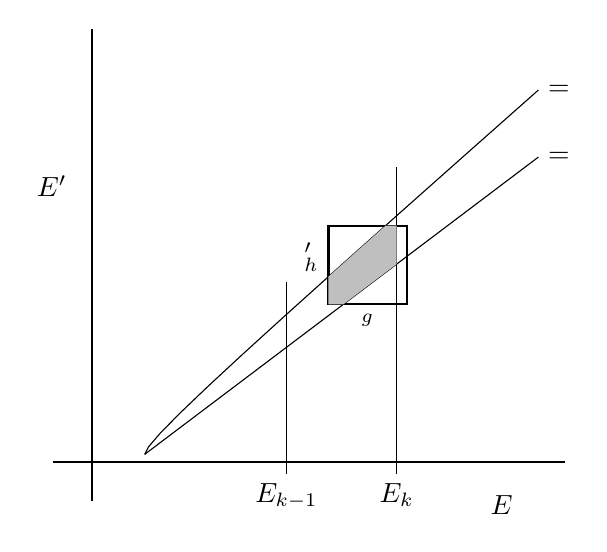
\begin{tikzpicture}
% the axes
  \draw[thick] (3.5,0) -- (10, 0);
  \draw[thick] (4,-0.5) -- (4, 5.5);
% the integration box
  \draw[thick](7,2) -- (7, 3) -- (8, 3) -- (8, 2) -- cycle;
% the data lines
  \draw (6.46667, -0.15) -- (6.46667, 2.28995);
  \node [below] at (6.46667, -0.15) {$E_{k-1}$};
  \draw (7.86667, -0.15) -- (7.86667, 3.74029);
  \node [below] at (7.86667, -0.15) {$E_{k}$};
% the curves
% mucm: -1
%\draw(4.66667, 0.0952381) --
%(4.71667, 0.0140642) --
%(4.86667, 0.00464791) --
%(5.11667, 0.0634261) --
%(5.46667, 0.187176) --
%(5.91667, 0.373109) --
%(6.46667, 0.618893) --
%(7.11667, 0.922636) --
%(7.86667, 1.28284) --
%(8.71667, 1.69832) --
%(9.66667, 2.16816);
% mucm: -0.5
%\draw(4.66667, 0.0952381) --
%(4.71667, 0.0735287) --
%(4.86667, 0.125453) --
%(5.11667, 0.24923) --
%(5.46667, 0.443248) --
%(5.91667, 0.706112) --
%(6.46667, 1.03666) --
%(7.11667, 1.43394) --
%(7.86667, 1.8972) --
%(8.71667, 2.42586) --
%(9.66667, 3.01946);
% mucm: 0
\draw(4.66667, 0.0952381) --
(9.66667, 3.87075);
% mucm: 0.5
\draw(4.66667, 0.0952381) --
(4.71667, 0.192458) --
(4.86667, 0.367064) --
(5.11667, 0.620838) --
(5.46667, 0.955391) --
(5.91667, 1.37212) --
(6.46667, 1.87219) --
(7.11667, 2.45654) --
(7.86667, 3.12593) --
(8.71667, 3.88094) --
(9.66667, 4.72204);
% mucm: 1
%\draw(4.66667, 0.0952381) --
%(4.71667, 0.251922) --
%(4.86667, 0.487869) --
%(5.11667, 0.806642) --
%(5.46667, 1.21146) --
%(5.91667, 1.70512) --
%(6.46667, 2.28995) --
%(7.11667, 2.96784) --
%(7.86667, 3.74029) --
%(8.71667, 4.60848) --
%(9.66667, 5.57333);
% integration region
\fill[gray!50] (7, 2) -- (7.0, 2.3517) -- 
(7.11667, 2.4565) -- (7.7256, 3) --
(7.86667, 3) -- (7.86667, 2.5116) --
(7.1892, 2) -- cycle;
% labels
 \node [below] at (9.2, -0.3) {$E$};
 \node [left] at (3.8, 3.5) {$E'$};
% \node [right] at (9.66667, 2.16816){$\mucm = -1$};
% \node [right] at (9.66667, 3.01946){$\mucm = -1/2$};
 \node [right] at (9.66667, 3.87075){$\mucm = \mucmjm$};
 \node [right] at (9.66667, 4.72204){$\mucm = \mucmj$};
% \node [right] at (9.66667, 5.57333){$\mucm = 1$};
 \node [left] at (7, 2.6){$\calE_h'$};
 \node [below] at  (7.5, 2){$\calE_g$};
\end{tikzpicture}
\caption{Integration region in the incident energy bin~$\calE_g$ and outgoing bin~$\calE_h'$
for probability data given at incident energies $E_{k-1}$ and~$E_k$ and direction
cosines $\mucmjm$ and~$\mucmj$ shown in the laboratory frame}
\label{Fig:2-body-region-lab}
\end{center} 

\end{figure}

\begin{figure}
% quadrature region in the (E, mucm) plane
\begin{center}
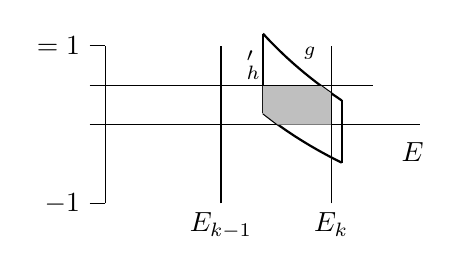
\begin{tikzpicture}
% the axes
  \draw (4.8,0) -- (9, 0);
  \draw (5,-1) -- (5, 1);
% the integration box
  \draw[thick] (7,0.1443) -- (7, 1.1547);
  \draw[thick] (8,-0.4841) -- (8, 0.3067);
% the curves
% Eout: 2
\draw[thick] (7, 0.144338) --
(7.1, 0.0661611) --
(7.2, -0.00780488) --
(7.3, -0.0779271) --
(7.4, -0.144528) --
(7.5, -0.207892) --
(7.6, -0.268272) --
(7.7, -0.325893) --
(7.8, -0.380958) --
(7.9, -0.433646) --
(8, -0.484123);
% Eout: 3
\draw[thick] (7, 1.1547) --
(7.1, 1.04855) --
(7.2, 0.948293) --
(7.3, 0.853396) --
(7.4, 0.763403) --
(7.5, 0.677908) --
(7.6, 0.596552) --
(7.7, 0.519015) --
(7.8, 0.445012) --
(7.9, 0.374288) --
(8, 0.306611);
% integration region
\fill[gray!50] (7, 0.1443) -- (7, 0.5) --
(7.7257, 0.5) -- (7.8, 0.445012) --
(7.86667, 0.3979) -- (7.86667, 0) --
(7.1894, 0) -- cycle;
% data lines
  \draw(4.8,0.5) -- (8.4, 0.5);
  \draw(6.46667, -1) -- (6.46667, 1);
  \node [below] at (6.46667, -1){$E_{k-1}$};
  \draw(7.86667, -1) -- (7.86667, 1);
  \node [below] at (7.86667, -1){$E_k$};
% labels
 \node [below] at (8.9, -0.1){$E$};
 \draw(4.8,-1) -- (5, -1);
 \node [left] at (4.8, -1){$-1$};
 \node [left] at (4.8, 0){$\mucmjm$};
 \node [left] at (4.8, 0.5){$\mucmj$};
  \draw(4.8,1) -- (5, 1);
 \node [left] at (4.8, 1){$\mucm = 1$};
 \node [left] at  (7.1, 0.75){$\calE_h'$};
 \node [above] at  (7.6, 0.7){$\calE_g$};
\end{tikzpicture}
\caption{Integration region of Fig.~\ref{Fig:2-body-region-lab} shown in center-of-mass coordinates}
\label{Fig:2-body-region-cm}
\end{center} 

\end{figure}

When the tabular data are interpolated by the method of cumulative
points of Section~\ref{Sec:cumProb}, the geometry is complicated by the
local unit-base transformations, but the basic ideas are the same.
Finally, for probability density data $g( \mucm \mid E)$ given as
Legendre coefficients in Eq.~(\ref{cmLegendre}), the only significant
difference is that the range of direction cosines becomes $-1 \le \mucm \le 1$
with the limitation that the energy $E$ of the outgoing particle lies in the
energy bin~$\calE_h'$.

\section{Format of data in the input file}
For tabulated probability density data $g( \mucm \mid E)$, the
data identifier as in Section~\ref{data-model}, is\\
  \Input{Process: two body transfer matrix}{}\\
and for the Legendre coefficients it is\\
  \Input{Process: Legendre two body transfer matrix}{}

\subsection{Data for both forms of probability density}
\label{Sec:2-body-data}
Because the boost from the center-of-mass frame to the laboratory
frame depends on the rest masses of the particles, these must be included
in the input file as described in Section~\ref{model-info}.  
For most reactions, the format for doing so is\\
  \Input{Projectile's mass:}{$\myi$} \\
 \Input{Target's mass:}{$\mtarg$} \\
 \Input{Product's mass:}{$\myo$} \\
 \Input{Reaction's Q value:}{$Q$} \\
The values of these quantities must be in the same units as
the energy bin boundaries.
The mass of the residual $\mres$ is then computed using
\begin{equation}
   \mres = \myi + \mtarg - \myo - Q.
 \label{2-body-mres}
\end{equation}

The mass of the residual may be given using the command\\
 \Input{Residual's mass:}{$\mres$}\\
but this is overridden by the result of Eq.~(\ref{2-body-mres})
unless the residual is a photon, $\mres = 0$.  In that case,
the value of $\myo$ is modified to enforce the
validity of Eq.~(\ref{2-body-mres}).

The code may use either Newtonian or relativistic mechanics in its
computations as specified in Section~\ref{Sec:relativistic}.  Relativistic
mechanics is used, however, if any of the particles involved in the reaction
is a photon.

The specifications that the energy $E$ of the incident particle is given in the laboratory
frame and the direction cosine $\mucm$ in the center-of-mass frame are,
Section~\ref{Reference-frame},\\
  \Input{Projectile Frame:  lab}{}\\
  \Input{Product Frame:  CenterOfMass}{}

\subsection{Angular probability density tables}
\label{Sec:angular-table}
The identification line for tabulated angular probability densities
is\\
  \Input{Angular data:}{$n = K$}\\
where $K$ is the number of incident energies~$E$.
This is followed by the interpolation rules for probability
densities from Section~\ref{interp-flags-probability}\\
  \Input{Incident energy interpolation:}{probability interpolation flag}\\
  \Input{Outgoing cosine interpolation:}{list interpolation flag}

There are then $K$ blocks, one for each incident energy $E_k$,\\
  \Input{Ein: $E_k$:}{$n = J_k$}\\
with $J_k$ pairs of values $\mucmj$ and $g(\mucm \mid E_k)$.  Thus,
with incident energy in MeV
a table of angular probability densities $g( \mucm \mid E)$ may look like\\
  \Input{Angular data:}{$n = 22$}\\
  \Input{Incident energy interpolation:}{lin-lin direct}\\
  \Input{Outgoing cosine interpolation:}{lin-lin}\\
  \Input{ Ein: 1.500000000000e-01 : n = 2}{}\\
   \Input{\indent -1.000000000000e+00  5.000000000000e-01}{}\\
    \Input{\indent 1.000000000000e+00  5.000000000000e-01}{}\\
  \Input{ Ein: 2.000000000000e-01 : n = 2}{}\\
  \Input{\indent  -1.000000000000e+00  4.550000000000e-01}{}\\
    \Input{\indent 1.000000000000e+00  5.450000000000e-01}{}\\
   \Input{\indent  } {$\cdots$}\\
  \Input{ Ein: 2.000000000000e+01 : n = 29}{}\\
   \Input{\indent -1.000000000000e+00  3.873180000000e-02}{}\\
  \Input{\indent  -9.500000000000e-01  2.943580000000e-02}{}\\
   \Input{\indent -9.000000000000e-01  2.582090000000e-02}{}\\
   \Input{\indent  } {$\cdots$}\\
    \Input{\indent 9.000000000000e-01  2.530490000000e+00}{}\\
   \Input{\indent 9.500000000000e-01  3.873180000000e+00}{}\\
    \Input{\indent 1.000000000000e+00  8.262750000000e+00}{}

\subsection{Legendre coefficients of angular probability density}
\label{Sec:2-bodyLegendreData}
Legendre coefficient data of the form Eq.~(\ref{cmLegendre})
for discrete 2-body reactions are given as\\
    \Input{Legendre coefficients:}{$n = K$}\\
where $K$ is the number of incident energies~$E$.
This is followed by the interpolation rule for simple lists
from Section~\ref{interp-flags-list}\\
  \Input{Interpolation:}{list interpolation flag}

The file closes with $K$ sets of data\\
    \Input{Ein: $E_k$:}{$n = L_k$}\\
with $L_k$ Legendre coefficients $c_\ell(E_k)$ for $\ell = 0$, 1,
\ldots\ , $L_k - 1$ in Eq.~(\ref{cmLegendre}).  With incident energy
in units of MeV, an example of this portion of the input file is\\
   \Input{Legendre coefficients: n = 17}\\
  \Input{Interpolation:}{lin-lin}\\
  \Input{  Ein: 1.843100e+00:  n = 3}{}\\
    \Input{\indent 1.000000e+00}{}\\
    \Input{\indent 0.000000e+00}{}\\
    \Input{\indent 0.000000e+00}{}\\
   \Input{\indent  } {$\cdots$}\\
  \Input{ Ein: 2.000000e+01:  n = 12}{}\\
    \Input{\indent 1.000000e+00}{}\\
    \Input{\indent 4.640500e-01}{}\\
    \Input{\indent 2.320700e-01}{}\\
    \Input{\indent 8.593700e-02}{}\\
    \Input{\indent 5.338700e-02}{}\\
    \Input{\indent 2.465600e-02}{}\\
    \Input{\indent -1.500600e-03}{}\\
    \Input{\indent -1.756300e-02}{}\\
   \Input{\indent  -1.108000e-02}{}\\
    \Input{\indent 1.931100e-02}{}\\
    \Input{\indent 1.150900e-02}{}\\
    \Input{\indent 5.643500e-03}{}

{
\newcommand{\Vacm}{\textbf{V}_{\text{1,cm}}}
\newcommand{\vacm}{V_{\text{1,cm}}}
\newcommand{\muacm}{\mu_{\text{1,cm}}}
\newcommand{\Valab}{\textbf{V}_{\text{1,lab}}}
\newcommand{\valab}{V_{\text{1,lab}}}
\newcommand{\Vbcm}{\textbf{V}_{\text{2,cm}}}
\newcommand{\Vblab}{\textbf{V}_{\text{2,lab}}}
\newcommand{\vblab}{V_{\text{2,lab}}}
\newcommand{\mualab}{\mu_{\text{1,lab}}}
\newcommand{\vbcm}{V_{\text{2,cm}}}
\newcommand{\mubcm}{\mu_{\text{2,cm}}}
\newcommand{\mayo}{m_{1,e}}
\newcommand{\mares}{m_{1,r}}
\newcommand{\mbyo}{m_{2,e}}
\newcommand{\mbres}{m_{2,r}}

\section{Two consecutive discrete 2-body reactions}
\label{Sec:2-step-2-body}
The \ENDFdata\ library~\cite{ENDFdata} contains data for one
reaction in the form of a sequence of two discrete 2-body reactions.
In this reaction, an incident deuteron hits a triton, with 
an outgoing excited ${}_2^4\text{He}$ nucleus and a neutron residual. 
The  excited ${}_2^4\text{He}$ nucleus then decays into a proton plus
a triton.  

\begin{figure}
% mapping to laboratory coordinates, 2-step, 2-body reactions, step 1
\begin{center}

\begin{tikzpicture}
% the triangle, step 1
  \draw[-{>[scale=2.5,
          length=5,
          width=3]},line width=0.4pt] (0, 0) -- (7.5, 3);
  \draw[-{>[scale=2.5,
          length=5,
          width=3]},line width=0.4pt] (0, 0) -- (6, 0);
  \draw[-{>[scale=2.5,
          length=5,
          width=3]},line width=0.4pt] (6, 0) -- (7.5, 3);
  \draw (6, 0) -- (8.2, 0);
  \draw (6.8, 0) arc (0: 63.43: 0.8);
  \draw ( 1.3, 0) arc (0: 21.8: 1.3);
% labels
  \node [below] at (3.5, -0.15) {$\Vtrans$};
  \node [above] at (4.2, 2) {$\Valab'$};
  \node [right] at (6.9, 1.4) {$\Vacm'$};
  \node [right] at (1.4, 0.3) {$\Theta_1$};
  \node [right] at (6.8, 0.45){$\theta_1$};
  \node [right] at (8.3, 2.7) {$\muacm = \cos \theta_1$};
  \node [right] at (8.3, 2) {$\mualab = \cos \Theta_1$};
  \node [above] at (7.5, 3) {$O'$};
  \node [left] at (0, 0) {$O$};
   \node [below] at (6, 0) {$C$};
\end{tikzpicture}
\caption{Step 1 of a 2-step 2-body reaction}
\label{Fig:2-step-2-body-step1}
\end{center} 

\end{figure}

In the current version of \gettransfer, the probability
density $g( \muacm \mid E)$ 
for the outgoing excited particle from the first step
must be represented as a table of Legendre
coefficients $c_\ell(E)$ 
for the expansion Eq.~(\ref{cmLegendre}).
The breakup second step is assumed
to be isotropic in the frame of the excited outgoing particle
from the first step.  A Newtonian analysis is given
here; see Appendix~\ref{Sec:2-step-2-body-rel} for a
relativistic version.

For the first step of the
reaction the masses are $\myi$ for the incident particle,
$\mtarg$ for the target, $\mayo$ for the outgoing particle 
which breaks up, and $\mares$ for the residual.  The $Q$-value
of the first step is denoted by~$Q_1$.

Figure~\ref{Fig:2-step-2-body-step1} illustrates
the notation used in analysis of the first step of this reaction.  
This figure is basically a copy of Figure~\ref{Fig:2-body-boost}.
In the discussion of
this figure, velocity vectors are denoted with bold 
face~$\textbf{V}$ and their
lengths with math italics~$V$.  

In Figure~\ref{Fig:2-step-2-body-step1}, the vector $\Vtrans$ 
is the velocity of the center of
mass for the first step of the reaction, and its magnitude is
as in Eq.~(\ref{Vtrans-length}).  For determination of the 
center-of-mass velocity $\vacm'$
of the excited outgoing particle from the first step,
Equation~(\ref{E_cm}) is modified to the form
$$
  \frac{\mayo ({\vacm'})^2}{2} =
    \frac{ \mtarg \mares E} { ( \myi + \mtarg ) ( \mayo + \mares ) } +
    \frac{ \mares Q_1} { ( \mayo + \mares ) },
$$
where $E$ is the energy of the incident particle and the
target is at rest.
If $\muacm$ is the direction cosine for~$\Vacm'$, 
then the velocity $\Valab'$ in the laboratory frame of the
excited outgoing particle from the first step satisfies the equation
$$
  ({\valab'})^2 = \vtrans^2 + ({\vacm'})^2 +
    2 \muacm \vtrans \vacm'.
$$

According to Eq.~(\ref{get_mu}), if $\valab' > 0$, then
the direction cosine~$\mualab$ is given by
\begin{equation*}
  \mualab  = \frac
   { \vtrans'  + \muacm  \vacm' }
    {\valab'}
\end{equation*}
For $\valab' = 0$, one may set $\mualab = 1$.

For the second (breakup) step, 
$\mbyo$ denotes the mass of the outgoing particle and
$\mbres$ the mass of the residual, and $Q_2$ is
the $Q$-value.  

Figure~\ref{Fig:2-step-2-body-step2} shows this second step
projected onto the plane determined by the vectors of the first step.
In this figure the full 3-dimensional geometry must be taken into
account because the emission is isotropic.  The point~$O'$ in the figure
identifies the center of mass of the breakup step.  An orthonormal 
$(\xi, \eta, \zeta)$-coordinate system
is introduced with origin at~$O'$. If $\valab' > 0$, the $\xi$-axis 
is chosen parallel to
the vector~$\Valab'$; otherwise, it is taken parallel to~$\Vtrans$.
If  the vectors $\Vtrans$ and~$\Valab'$ generate a plane, then
the $\eta$-axis is selected to lie in this plane.  For colinear
$\Vtrans$ and~$\Valab'$, the $\eta$-axis may be in any direction
perpendicular to the $\xi$-axis.
The $\zeta$-axis is chosen perpendicular to the $(\xi, \eta)$-plane.
  
In this reference frame the magnitude of the
velocity~$\Vbcm'$ of the outgoing
particle from the breakup step is obtained from Equation~(\ref{E_cm})
as
$$
  \frac{\mbyo (\vbcm')^2}{2} =
    \frac{ \mbres Q_2} { ( \mbyo + \mbres ) }.
$$
Because the breakup is isotropic, the vector~$\Vbcm'$ in 
Figure~\ref{Fig:2-step-2-body-step2} 
with tail at~$O'$ has its head uniformly distributed on
the sphere~$\Sigma_0$.  For a fixed $\Valab'$ and angle~$\theta_2$
between $\Vbcm'$ and the $\xi$-axis, the head of~$\Vbcm'$ lies
on a circle on~$\Sigma_0$, which is projected as the line segment from
$A$ to~$B$ in  Figure~\ref{Fig:2-step-2-body-step2}.
The magnitude~$\vblab'$ of the velocity of the final emitted
particle is the same for all vectors~$\Vbcm'$ with heads on
the segment from $A$ to~$B$, and in the case that the head is
at~$B$ it is clear that
\begin{equation}
  ({\vblab'})^2 = (\valab')^2 + (\vbcm')^2 +
    2 \mubcm \valab' \vbcm',
 \label{2-step-2-body-V}
\end{equation}
where $\mubcm = \cos \theta_2$.
Furthermore, the energy of the final outgoing particle in the
laboratory frame is
\begin{equation}
  \Elab' = \frac{ \mbyo (\vblab')^2 }{2}.
 \label{2-step-2-body-E}
\end{equation}

For this 2-step reaction, in the computation of the
elements of the transfer matrix Eq.~(\ref{muEint}) is
replaced by
\begin{equation}
    \Inum_{g,h,\ell} =
     \int_{\calE_g} dE \, \sigma ( E ) w(E) \widetilde \phi_\ell(E) 
    \int_{\muacm} d\muacm  \, g(\muacm \mid E)
    \int_{\Sigma_{0,h}} d\sigma_0 \, P_\ell( \mulab ).
  \label{2-step-muEint}
\end{equation}
In this integral $\Sigma_{0,h}$ is the subset of $\Sigma_0$ on which
$\Elab'$ from Eqs.~(\ref{2-step-2-body-V}) and~(\ref{2-step-2-body-E})
lies in the outgoing energy bin~$\calE_h'$,
and $d\sigma_0$ is the differential surface area
on the sphere~$\Sigma_0$ normalized so that
$$
  \int_{\Sigma_0} d\sigma_0 = 1.
$$

The direction cosine~$\mulab$ in Eq.~(\ref{2-step-muEint})
is obtained from
\begin{equation}
  \Vblab' \cdot \Vtrans = \mulab  \vblab' \vtrans.
  \label{2-step-mulab}
\end{equation}
The geometry used in the computation of $\mulab$ is illustrated
in Figure~\ref{Fig:2-step-2-body-step2}.  
This figure shows a case in which
$\Vbcm'$ lies outside of the $(\xi, \eta)$-plane.  The
$\zeta$-component of~$\Vbcm'$ is orthogonal to~$\Vtrans$,
so it suffices to work with the projection of $\Vbcm'$ onto
the $(\xi, \eta)$-plane in the computation of~$\mulab$
in Eq.~(\ref{2-step-mulab}).  Consequently, if $\vblab' > 0$, it easily seen that
\begin{equation}
  \mulab = \frac{ \mualab ( \valab' + \xi ) - \eta \sqrt{ 1 - \mualab^2 } }
             { \vblab'}.
  \label{2-step-mulab-xi}
\end{equation} 
For $\vblab' = 0$, the value of~$\mulab$
is taken as~$\mulab = 1$.

\begin{figure}
% mapping to laboratory coordinates, 2-step, 2-body reactions
\begin{center}

\begin{tikzpicture}
% the triangle, step 1
  \draw[-{>[scale=2.5,
          length=5,
          width=3]},line width=0.4pt] (0, 0) -- (7.5, 3);
  \draw[-{>[scale=2.5,
          length=5,
          width=3]},line width=0.4pt] (0, 0) -- (6, 0);
\draw (6, 0) -- (9, 0);
\draw ( 1.3, 0) arc (0: 27.1: 1.3);
% step 2
 \draw (7.5, 3) -- (10, 4);
 \draw (9.3, 3) arc (0: 360: 1.8);
   \draw[-{>[scale=2.5,
          length=5,
          width=3]},line width=0.4pt] (7.5, 3) -- (8.3, 4.25);
   \draw[-{>[scale=2.5,
          length=5,
          width=3]},line width=0.4pt] (0, 0) -- (8.3, 4.25);
  \draw (7.779, 2.868) -- (9.117, 2.209);
  \draw (8.125, 4.688) -- (9.117, 2.209);
  \draw (7.5, 3) -- (9.117, 2.209);
  \draw (6.5, 5.5) -- (8.4, 0.75);
 \draw (7.949, 2.78) arc (-26.1: 21.8: 0.5);
  \draw ( 2.3, 0) arc (0: 21.8: 2.3);
% labels
  \node [below] at (3.5, -0.15) {$\Vtrans$};
  \node [below] at (4, 1.4) {$\Valab'$};
  \node [right] at (6.5, 0.9) {$\Sigma_0$};
  \node [above] at (4, 2.2) {$\Vblab'$};
  \node [right] at (7.9, 3.5) {$\Vbcm'$};
  \node [right] at (8, 3){$\theta_2$};
  \node [right] at (1.3, 0.3){$\Theta_0$};
  \node [right] at (2.3, 0.4) {$\Theta_1$};
  \node [below] at (9.9, 3.95) {$\xi$};
  \node [left] at (6.5, 5.2) {$\eta$};
  \node [above] at (8.125, 4.688) {$A$};
  \node [below] at (9.3, 2.3) {$B$};
  \node [below] at (7.35, 2.9) {$O'$};
  \node [left] at (0, 0) {$O$};
  \node [right] at (0.2, 5) {$\mubcm = \cos \theta_2$};
  \node [right] at (0.2, 4.4) {$\mualab = \cos \Theta_1$};
  \node [right] at (0.2, 3.8) {$\mulab = \cos \Theta_0$};
%  \node [below] at (6, 0) {$C$};
\end{tikzpicture}
\caption{Step 2 for a 2-step 2-body reaction}
\label{Fig:2-step-2-body-step2}
\end{center} 

\end{figure}

It remains to identify the set~$\Sigma_{0, h}$ in the integral
Eq.~(\ref{2-step-muEint}).
In terms of the coordinate~$\zeta$, the surface of the sphere~$\Sigma_0$ may
be written as
\begin{equation}
  \zeta = \pm \sqrt{
     (\vbcm')^2 - \xi^2 - \eta^2 }
     \quad \text{for $\xi^2 + \eta^2 \le (\vbcm')^2.$}
  \label{2-step-Sigma-xi}
\end{equation} 
Because of the mirror symmetry in the $(\xi, \eta)$ plane, it suffices to work with the
positive square root
\begin{equation}
  \zeta = \sqrt{
     (\vbcm')^2 - \xi^2 - \eta^2 }
     \quad \text{for $\xi^2 + \eta^2 \le (\vbcm')^2.$}
  \label{2-step-def-zeta}
\end{equation}
The energy
$\Elab'$ in Eq.~(\ref{2-step-2-body-E}) may lie in the outgoing 
energy bin~$\calE_h'$ for fixed incident energy~$E$
and for step~1 direction cosine~$\muacm$.  If it does so
for at least 2 values of the step~2 direction cosine~$\mubcm$,
then $\Elab'$ is in~$\calE_h'$ for $\mubcm$
on an interval
\begin{equation}
  a_h \le \mubcm \le b_h
  \label{2-step-ab-range}
\end{equation}
with
$$
  -1 \le a_h < b_h \le 1.
$$
Consequently, for the hemisphere in Eq.~(\ref{2-step-Sigma-xi}) the integral
over $\Sigma_{0,h}$ in Eq.~(\ref{2-step-muEint}) may be written as
\begin{equation}
   \int_{\Sigma_{0,h}} d\sigma_0 \, P_\ell( \mulab ) =
   \frac{1}{2 \pi \vbcm' }
   \int_{ a_h \vbcm}^{b_h \vbcm} d\xi \int_{- \sqrt{ (\vbcm')^2 - \xi^2 }}
                           ^{\sqrt{ (\vbcm')^2 - \xi^2 }} d\eta \,
          \frac {P_\ell( \mulab ) } { \sqrt{ (\vbcm')^2 - \xi^2 - \eta^2}}.
  \label{2-step-Sigma-int}
\end{equation}
In this integral the change of variables
\begin{alignat}{2}
  \xi &= \vbcm' \, \mubcm 
    \quad &\text{for $a_h \le \mubcm \le b_h$,}
      \label{2-step-def-xi} \\
  \eta &= \vbcm' \sqrt{ 1 - \mubcm^2 } \, \sin w 
    \quad &\text{for $-\pi/2 \le w \le \pi/2$}
  \label{2-step-def-eta}
\end{alignat}
leads to the relation
\begin{equation}
   \int_{\Sigma_{0,h}} d\sigma_0 \, P_\ell( \mulab ) =
   \frac{1}{2 \pi }
   \int_{ a_h}^{b_h} d\mubcm \int_{- \pi/2}
                           ^{\pi/2} dw \,
          P_\ell( \mulab ) .
 \label{2-step-int-sigma}
\end{equation}
This representation is used in the calculation of the
subintegral over $\Sigma_{0,h}$ in Eq.~(\ref{2-step-muEint}).

\subsection{The input file for a 2-step 2-body reaction}
In the input file to \gettransfer, the identifier for this reaction is\\
  \Input{Process: two step two body reaction}{}\\
The particle masses and the $Q$-values for this reaction are
given by\\
 \Input{Target's mass:}{$\mtarg$}\\ 
 \Input{Projectile's mass:}{$\myi$}\\
 \Input{First residual's mass:}{$\mares$}\\
 \Input{First product's mass:}{$\mayo$}\\
 \Input{First step's Q value:}{$Q_1$}\\
 \Input{Second product's mass:}{$\mbyo$}\\
 \Input{Second residual's mass:}{$\mbres$}\\ 
 \Input{Second step's Q value:}{$Q_2$}\\
The mass $\mayo$ of the excited outgoing particle
from the first step is recalculated using
\begin{equation}
   \mayo = \myi + \mtarg - \mares - Q_1.
 \label{2-step-mayo}
\end{equation}
This is because the values on the right-hand side
of Eq.~(\ref{2-step-mayo}) are usually known to high accuracy.
In addition, the value of $Q_2$ is computed using
$$
  Q_2 = \mayo - \mbyo - \mbres.
$$

For the first step of the reaction, the Legendre
coefficients $c_\ell(E)$ for the expansion 
Eq.~(\ref{cmLegendre}) of the probability
density $g( \muacm \mid E)$ 
for the outgoing excited particle are given as
in Section~\ref{Sec:2-bodyLegendreData}.

An example of the model-dependent portion of the input
file, Section~\ref{model-info}, is as follows.\\
 \Input{Target's mass:  2.808921000497e+03}{}\\
 \Input{Projectile's mass:  1.876124078321e+03}{}\\
 \Input{First residual's mass: 939.565413016980301}{}\\
 \Input{First product's mass: 3747.70426580102}{}\\
  \Input{First step's Q value: -2.2246}{}\\
 \Input{Second product's mass: 938.782992507523659}{}\\
 \Input{Second residual's mass:  2.808921000497e+03}{}\\
 \Input{Second step's Q value: 0.0002728}{}\\
\vskip 5pt
 \Input{Legendre coefficients: n = 30}{}\\
 \Input{Interpolation: lin-lin}{}\\
 \Input{ Ein: 3.71:  n = 3}{}\\
  \Input{ \indent 1.0}{}\\
  \Input{ \indent 0.0}{}\\
  \Input{ \indent 0.0}{}\\
 \Input{ Ein: 3.9:  n = 3}{}\\
  \Input{ \indent 1.0}{}\\
  \Input{ \indent -0.14079}{}\\
  \Input{ \indent 0.026804}{}\\
    \Input{ $\cdots$}{}\\
  \Input{ Ein: 10.0:  n = 3}{}\\
  \Input{ \indent 1.0}{}\\
  \Input{ \indent 0.24417}{}\\
  \Input{ \indent 0.011232}{}\\
}
